%% The following is a directive for TeXShop to indicate the main file
%%!TEX root = diss.tex

\chapter{Introduction}
\label{ch:Introduction}

%%%%%%%%%%%%%%%%%%%%%
\begin{figure}
    \centering
  %  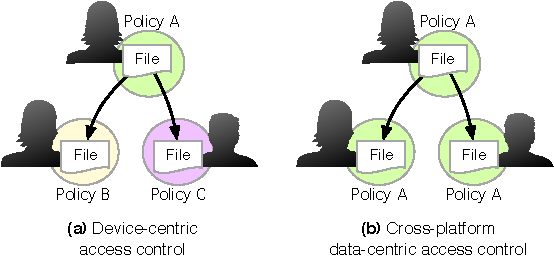
\includegraphics[width=\columnwidth]{fig/tcapsules-contrast.pdf}
    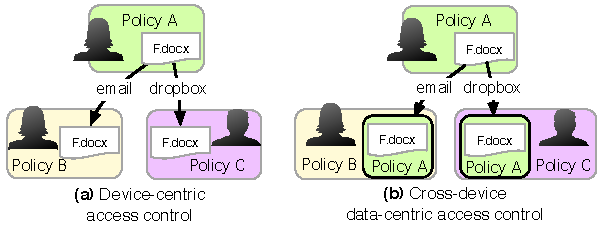
\includegraphics[width=\columnwidth]{fig/tcapsules-contrast2.pdf}
    \caption{(a) Today, a data creator has no control over their data on remote
      devices: devices enforce local policies on data they receive. We propose (b)
      cross-platform policies that move with data and are enforced uniformly
      across devices.}
    \label{fig:ControlBoundaries}
  \end{figure}
  %%%%%%%%%%%%%%%%%%%%%/
  
Modern mobile devices are highly capable and have enabled users to create and
  share rich content such as videos, pictures, and documents. However, users often have little control over their shared data. As illustrated in
  Figure~\ref{fig:ControlBoundaries}, a user has full control over her file as long as it stays on her device. She loses this control the moment the file leaves her device boundaries. For example, files backed up to iCloud or Dropbox are vulnerable to the security of those platforms and files shared with other users are vulnerable to their benevolence and their device security policies.
  
  Users today rely on ad-hoc solutions. For example, they might use
  Cryptomator \cite{cryptomator} to encrypt their files before backing them up to the cloud
  or SnapChat to send self-destructing images that are viewable only for
  a limited period of time \cite{snapchat}. These apps address particular use-cases with
  coarse controls and do not provide any general-purpose data protection
  mechanisms.
  
  Existing work has proposed several solutions to let users retain control over their data as it crosses device boundaries. A current
  state of the art approach is to use a hardware-based trusted
  execution environment (TEE) to control accesses to sensitive files.
  The focus is to ensure that users retain {\em full} control over their shared data. DroidVault~\cite{li14droidvault}, for example, does not allow regular apps running outside the TEE to access the data. Instead, it requires data owners to explicitly write and whitelist the code that is allowed to process sensitive data, and it executes this code within the TEE. We believe that such restrictions make the corresponding systems impractical. Users already trust and rely on a variety of apps to create and share content. It is unlikely
  that users would use a system that does not support their apps.
  
  We present a platform-level file protection mechanism that does not restrict users into using certain apps. To achieve this, we rely on a pragmatic pessimistic-optimistic threat model. In the pessimistic state, we consider the device and apps completely untrusted and rely on a TEE to perform safety checks. When it is considered safe, the
  system transitions into the optimistic state where we also trust the
  OS kernel and the app accessing sensitive data. Finally, when the app no longer uses the data, the system switches back into the pessimistic state. We leave a further discussion of our threat model to Section~\ref{ch:ThreatModel}.
  
  We contribute {\bf Trusted Capsules}, a data-centric access control abstraction that provides a mechanism to protect against this threat model. It enables users to bundle sensitive files with
  flexible policies that govern their accesses into encrypted units we call {\em
    capsules}. Each capsule appears in the system as a regular file. When an app
  attempts to open a capsule, the platform evaluates the policy in a TEE. If the
  the policy allows the access, the capsule's contents are unsealed (decrypted) and
  provided to the app and are resealed (re-encrypted) when the app later closes
  the file. In our prototype, we use ARM TrustZone as the TEE and design policies
  as stateful programs that can base access decisions on information such as
  location, time, or the number of prior accesses and may, if necessary, modify
  the data itself (e.g., for redaction).

  Our contributions may be summarized as follows:

\begin{itemize}

\item A pragmatic access control abstraction for protecting sensitive files
  across device boundaries that works with existing unmodified apps.

\item Using our prototype, we show that our proposed approach imposes slowdowns
  only when a capsule is being opened or closed (An overhead of 1.96x and 1.67x, respectively,
  in the absence of any real security policy). Once a capsule file is open, data can be read at a
  throughput identical to reading regular files.

\end{itemize}

\endinput

Any text after an \endinput is ignored.
You could put scraps here or things in progress.
